\documentclass{beamer}
%\usetheme{Ilmenau}
%\usecolortheme{beaver}

\usepackage[slovak,american]{babel}
\usepackage[utf8]{inputenc}
\usepackage{graphicx}
\usepackage{adjustbox}
 \usepackage{xcolor}
 
 \newsavebox\MBox
\newcommand\Cline[2][red]{{\sbox\MBox{$#2$}%
  \rlap{\usebox\MBox}\color{#1}\rule[-2.2\dp\MBox]{\wd\MBox}{1pt}}}

%\usefonttheme{serif}

\definecolor{UKOrange}{HTML}{ef9424} %
\definecolor{UKBrown}{HTML}{a96d5e} %
\definecolor{UKLight}{HTML}{d8b6ab} %
\definecolor{UKDark}{HTML}{7a4f44}
\definecolor{UKDarker}{HTML}{4d312b} 
\definecolor{UKDarkest}{HTML}{2e1e1a}
\definecolor{UKRed}{HTML}{bf1f1c}

\setbeamertemplate{footline}[frame number]{}
\setbeamertemplate{navigation symbols}{}

%\usecolortheme{beaver}
\setbeamertemplate{itemize item}[square]
\setbeamercolor{itemize item}{fg = UKBrown}
\setbeamercolor{itemize subitem}{fg = UKLight}
\setbeamercolor{enumerate item}{fg = UKDark}

\setbeamercolor{footnote}{fg=UKLight}
\setbeamercolor{footnote mark}{fg=UKLight}
\setbeamerfont{footnote}{size=\tiny}
\renewcommand\footnoterule{}

\usetheme{default}
\beamertemplatenavigationsymbolsempty
\setbeamercolor{title}{fg=white, bg=UKBrown}
\setbeamercolor{frametitle}{fg=white, bg=UKBrown}
\setbeamercolor{block title}{bg=UKBrown, fg= white}
\setbeamercolor{block body}{bg =UKLight, fg = UKDarkest}

\useoutertheme[subsection=false]{miniframes}
\AtBeginSection[]{\subsection{}}

\setbeamercolor{below lower separation line head}{bg=UKDark}
\addtobeamertemplate{headline}{}{%
  \begin{beamercolorbox}[colsep=0.5pt]{below lower separation line head}
  \end{beamercolorbox}
}
%\setbeamercolor*{mini frame}{fg=white,bg=UKRosy}
\setbeamercolor{section in head/foot}{fg=UKLight, bg=UKDark}

%\setbeamertemplate{itemize/enumerate body begin}{\normalsize}
%\setbeamertemplate{itemize/enumerate subbody begin}{\normalsize}




%\newcommand{\codeblock}[2]{ \begin{block}{#1} \begin{verbatim}#2\end{verbatim}\end{block}}

%\defbeamertemplate*{title page}{customized}[1][]
%{
%  \begin{centering}
%    \begin{beamercolorbox}[sep=8pt,center]{title}
%      \usebeamerfont{title}\inserttitle
%    \end{beamercolorbox}
%  \end{centering}
%  \bigskip
%
%\begin{columns}[onlytextwidth,T]
%
%
%  \column{27mm}
%  \includegraphics[width=27mm]{images/logoFMFI.png}
%  
%  \column{\dimexpr\linewidth-54mm-6mm}
%  \centering
%  \vspace{5mm}  
%  \usebeamerfont{author}\insertauthor\par
%  \vspace{5mm}
%  \usebeamerfont{institute}\insertinstitute\par
%
%  \column{27mm}
%  \includegraphics[width=27mm]{images/logoUK.png}  
%\end{columns}
%\centering
%\vspace{7mm}
%  \usebeamerfont{date}\insertdate\par
%}

\DeclareMathOperator*{\argmax}{arg\,max}


\title[Stromy]{Rozpoznávanie obrazcov - 9. cvičenie \\ Naivný Bayesov klasifikátor}
\author[Viktor Kocur]{Viktor Kocur \\{\small viktor.kocur@fmph.uniba.sk}}
\institute{DAI FMFI UK}
\date{21.4.2020}
%\titlegraphic{\includegraphics[width=2.7cm]{images/logoFMFI.png}\hspace*{1cm}~%
%   \includegraphics[width=2.7cm]{images/logoUK.png}
%}


\begin{document}
\selectlanguage{slovak}

\begin{frame}[plain]
  \titlepage  
\end{frame}

\section{Naivný Bayes}

\begin{frame}
\frametitle{Bayesovo pravidlo}
\begin{block}{Bayesovo pravidlo}
Budeme opäť používať Bayesovo pravidlo:
\begin{equation}
P(\omega_i | \vec{x}) = \frac{P(\vec{x}|\omega_i) P(\omega_i)}{P(\vec{x})}
\end{equation}
\end{block}

\begin{block}{Naivita}
Náš klasifikátor je naivný a predpokladá, že príznaky sú nezávislé:
\begin{equation}
P(\vec{x}|\omega_i) = \prod_{k} P(x_k | \omega_i)
\end{equation}
\end{block}
\end{frame}


\begin{frame}
\frametitle{Klasifikátor}
\begin{block}{Klasifikácia}
Klasifikujeme pomocou nájdenia triedy s najväčšou pravdebodobnosťou:
\begin{align}
pred_i &= \argmax_i \left( \frac{P(\vec{x}|\omega_i) P(\omega_i)}{P(\vec{x})} \right) \\
          &= \argmax_i \left(P(\vec{x}|\omega_i) P(\omega_i) \right) \\
          &= \argmax_i \left(P(\omega_i) \prod_{k} P(x_k | \omega_i) \right)
\end{align}
\end{block}
\end{frame}


\begin{frame}
\frametitle{Klasifikátor}
\begin{block}{Výpočet hodnôt}
Budeme predpokladať že máme kategorické príznaky. Teda pre každé $k$ môže $x_k$ nadobúdať iba konečne mnoho diskrétnych hodnôt. Označíme celkový počet prvkov trénovacej množiny ako $N$. Počet prvkov, ktoré patria do triedy $\omega_i$ ako $N_i$. Počet prvkov, ktoré patria do $\omega_i$ a pre $k$-tý príznak majú hodnotu $v$ ako $N_{i,k,v}$. Potom môžeme definovať:
\begin{gather}
P(\omega_i) = \frac{N_i}{N} \\
P(x_k = v | \omega_i) = \frac{N_{i,k,v}}{N_i} 
\end{gather}
\end{block}
\end{frame}

\begin{frame}
\frametitle{Klasifikátor}
\begin{columns}[onlytextwidth,T]


  \column{70mm}
  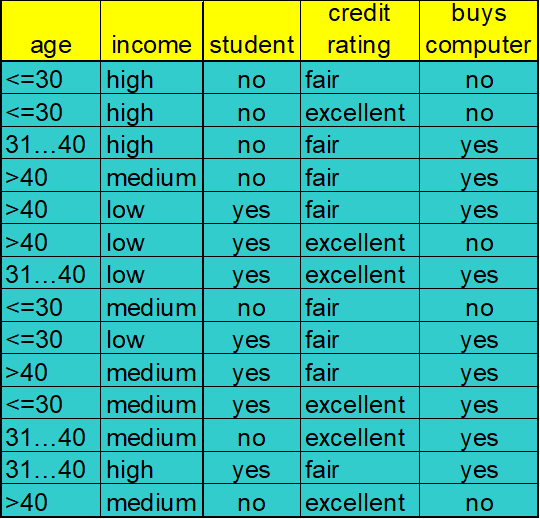
\includegraphics[width=70mm]{table.png}
  
  \column{30mm}
  \begin{block}{Úloha}
  Spočítajte do ktorej kategórie bude patriť zákazník s náhodnými prediktormi.
  \end{block}
\end{columns}

\end{frame}


\begin{frame}
\frametitle{Klasifikátor}
\begin{block}{Nekategorické dáta}
V prípade, že niektorý príznak je numerický, tak nemôžeme aplikovať výpočet z predchádzajúceho slidu. Preto budeme pravdepodobnosť $P(x_k | \omega_i)$ odhadovať nejakou distribučnou funkciou. 
\end{block}

\begin{block}{Parametrické metódy}
Pri parametrických metódach odhadneme parametre nejakého dopredu určeného rozdelenia.
\end{block}

\begin{block}{Neparametrické metódy}
Pri neparametrických metódach pravdepodobnosť vypočítame na základe bodov z trénovacej množiny v okolí bodu o ktorý sa zaujímame.
\end{block}
\end{frame}

\begin{frame}
\frametitle{Matlab}
\begin{block}{fitcnb}
Mdl = fitcnb(T,'nazov\_pola') - vráti naivný Bayesov klasifikátor pre tabuľku T pre klasifikačný cieľ pre stĺpec nazov\_pola.
\end{block}


\begin{block}{Malab - Table dátový typ}
Pre prácu s tabuľkami si pozrite: \\
\url{https://www.mathworks.com/help/matlab/tables.html}\\
\vspace{1em}
A dôležitá je aj časť o prístup k dátam:
\url{https://www.mathworks.com/help/matlab/matlab_prog/access-data-in-a-table.html}
\end{block}
\end{frame}

\begin{frame}[fragile]
\frametitle{Naivný Bayes na tabuľkových dátach}
\begin{block}{Na dátach}
\begin{verbatim}
load census1994
Mdl = fitcnb(adulddata, 'salary');\end{verbatim}
\end{block}

\begin{block}{Úloha}
Zistite presnosť klasifikátora tak, že ho spustíte (Mdl.predict) na tabuľku adulttest a porovnáte výsledok.
\end{block}
\end{frame}

\begin{frame}
\frametitle{Matlab}
\begin{block}{fitcnb}
Mdl = fitcnb(X,y) - vráti naivný Bayesov klasifikátor
\end{block}

\begin{block}{Úloha}
Otestujte naivný Bayesov klasifikátor na fisheriris dátach.
\end{block}

\begin{block}{Úloha}
Zobrazte si klasifikátor na dátach zo 6. cvičenia pomocou úpravy skriptu showSVM z toho istého cvičenia.
\end{block}
\end{frame}

\end{document}